\documentclass[12pt]{article}
\usepackage{graphicx}
\usepackage{float}
\usepackage{amsmath}
\begin{document}
\title{Electrical Engineering 113, Bonus Project}
\date{June 14th, 2019}
\author{Michael Wu\\UID: 404751542}
\maketitle

\section{Given Information}

Let \(\mathbf{x} = (2,y)\) be the position of the source, \(\mathbf{x}_1 = (0,4)\)
be the position of the first receiver, and \(\mathbf{x}_2 = (0,4.5)\) be the position
of the second receiver. Let \(P_{r,l}\) be the power received by the \(l\)th receiver,
\(P_t\) be the power at the source, and \(y_l\) be the \(y\) coordinate of the \(l\)
receiver. We model the received power with the following formula.
\[P_{r,l}=\frac{P_t}{4 + (y-y_l)^2}\]

\section{Normalizing Noise}

Assume the noise in the received power signal is log-normal distributed, so we can take the logarithm
and rewrite this as follows.
\begin{align*}
    \ln(P_{r,l})-\ln(P_t)&=-\ln\left(4 + (y-y_l)^2\right) + n_l\\
    r_l&=-\ln(d_l^2) + n_l\\
    r_l&=-2\ln(d_l) + n_l
\end{align*}
Now we can assume the noise \(n_l\) follows a Gaussian distribution \(N(0,\lambda_l^2)\).
Here we have \(r_l=\ln(P_{r,l})-\ln(P_t)\) and \(d_l\) is the distance formula from the
source to the receiver.

\section{Matrix Formulation}

Letting \(R=4+y^2\), we can rewrite the distance formula as follows.
\begin{align*}
    d_l^2&=4 + (y-y_l)^2\\
    &=4 + y^2 - 2yy_l + y_l^2\\
    R - 2yy_l&=d_l^2-y_l^2
\end{align*}
Equivalently in matrix form this is the following.
\[\begin{bmatrix}-2\times4 & 1\\-2\times4.5 & 1\end{bmatrix}\begin{bmatrix}y\\R\end{bmatrix}
=\begin{bmatrix}d_1^2-4^2\\d_2^2-4.5^2\end{bmatrix}\]

\section{Unbiased Distance Estimator}

Since we do not know \(d_l^2\), can try to obtain an estimate of it using the following calculations.
\begin{align*}
    r_l&=-2\ln(d_l) + n_l\\
    \ln(d_l)&=\frac{n_l-r_l}{2}\\
    d_l &= e^{\frac{n_l-r_l}{2}}\\
    d_l^2 &= e^{n_l-r_l}
\end{align*}

Let \(x=n_l-r_l\) be a random variable that is normally distributed with a mean at \(-r_l\)
and the variance \(\lambda_l^2\) coming entirely from \(n_l\). We calculate the expected value
of \(d_l^2\) as follows.
\begin{align*}
    E\left[e^{n_l-r_l}\right] &= E\left[e^x\right]\\
    &=\int e^x \frac{1}{\sqrt{2\pi\lambda_l^2}}e^{-\frac{1}{2}\frac{(x+r_l)^2}{\lambda_l^2}}\,dx
\end{align*}
We can make the change of variables \(x=z\lambda_l - r_l\) in order to make the integral easier
to evaluate.
\begin{align*}
    E\left[e^x\right] &= \int e^{z\lambda_l - r_l}\frac{1}{\sqrt{2\pi\lambda_l^2}}e^{-\frac{1}{2}z^2}\lambda_l\,dz\\
    &=e^{-r_l}\int e^{z\lambda_l}\frac{1}{\sqrt{2\pi}}e^{-\frac{1}{2}z^2}\,dz\\
    &=e^{-r_l}\int \frac{1}{\sqrt{2\pi}}e^{z\lambda_l-\frac{1}{2}z^2}\,dz\\
    &=e^{-r_l}\int \frac{1}{\sqrt{2\pi}}e^{\frac{1}{2}\lambda_l^2 - \frac{1}{2}(z-\lambda_l)^2}\,dz\\
    &=e^{-r_l}e^{\frac{1}{2}\lambda_l^2} \int\frac{1}{\sqrt{2\pi}}e^{-\frac{1}{2}(z-\lambda_l)^2}\,dz\\
    &=e^{-r_l+\frac{1}{2}\lambda_l^2}
\end{align*}
The integral evaluates to \(1\) because it is the integral of a normal distribution. We can substitute
this expression into the matrix formulation of the problem since it is an unbiased estimator of \(d_l^2\).
\[\begin{bmatrix}-2\times4 & 1\\-2\times4.5 & 1\end{bmatrix}\begin{bmatrix}y\\R\end{bmatrix}
=\begin{bmatrix}e^{-r_1+\frac{1}{2}\lambda_1^2}-4^2\\e^{-r_2+\frac{1}{2}\lambda_2^2}-4.5^2\end{bmatrix}\]

\section{Polynomial Formulation}

We can expand the matrix formulation of the problem to obtain the following equations.
\begin{align*}
    y^2-8y+20-e^{-r_1+\frac{1}{2}\lambda_1^2}&=0\\
    y^2-9y+24.25-e^{-r_2+\frac{1}{2}\lambda_2^2}&=0\\
    y-4.25-e^{-r_1+\frac{1}{2}\lambda_1^2}+e^{-r_2+\frac{1}{2}\lambda_2^2}&=0\\
    y&=4.25+e^{-r_1+\frac{1}{2}\lambda_1^2}-e^{-r_2+\frac{1}{2}\lambda_2^2}
\end{align*}
This is a closed form solution for \(y\), so all we need to do is obtain the variances
and \(r_1\) and \(r_2\).

\section{Code Implementation}

Obtaining \(r_1\) and \(r_2\) from our data is straightforward. We will take the average power over
intervals of a whole period which is one second or 200 samples at a time. By doing this we are able
to reduce the effect of noise. The following code generates the power in log form.
\begin{verbatim}
window=200;
N=length(transmitted_signal)-window;
power1=zeros(1,N);
power2=zeros(1,N);
powerT=zeros(1,N);
tPrime=zeros(1,N);
for i=1:N
    indices=i:i+window;
    power1(i)=log(mean(received_signal1(indices).^2));
    power2(i)=log(mean(received_signal2(indices).^2));
    powerT(i)=log(mean(transmitted_signal(indices).^2));
    tPrime(i)=mean(t(indices));
end
\end{verbatim}
Since our given data contains only noise from \(-5\leq t \leq 0\), we can use those data points to
obtain the variances \(\lambda_1\) and \(\lambda_2\) with the following code.
\begin{verbatim}
var1=var(power1(1:1000-window));
var2=var(power2(1:1000-window));
\end{verbatim}
Finally we can calculate the expression for \(y\) with the following code.
\begin{verbatim}
r1=power1-powerT;
r2=power2-powerT;
y=4.25+exp(-r1+var1/2)-exp(-r2+var2/2);
\end{verbatim}
We can also smooth the data so it is easier to work with. I found the following
moving average filter with window size 50 worked well.
\begin{verbatim}
y=smoothdata(y,'movmean',50);
\end{verbatim}
This results in the following unsmoothed and smoothed signals.
\begin{figure}[H]
    \begin{center}
        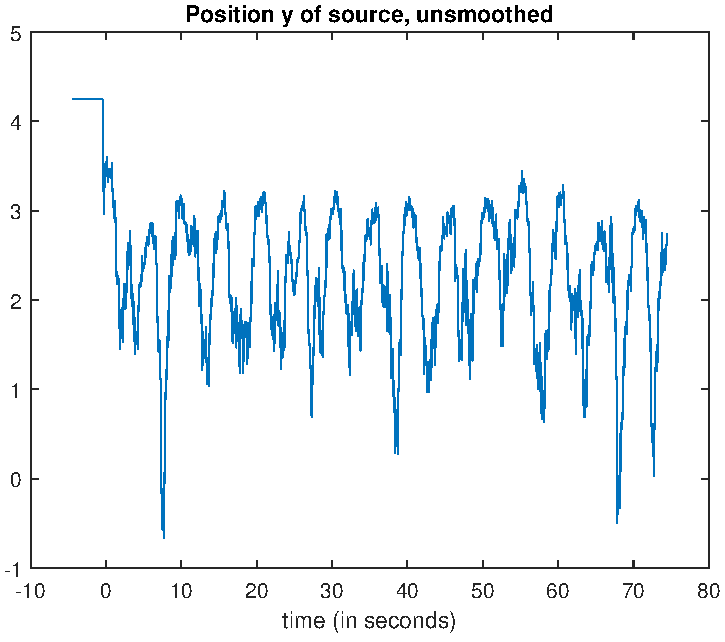
\includegraphics[width=2.5in]{y-unsmoothed.pdf}
        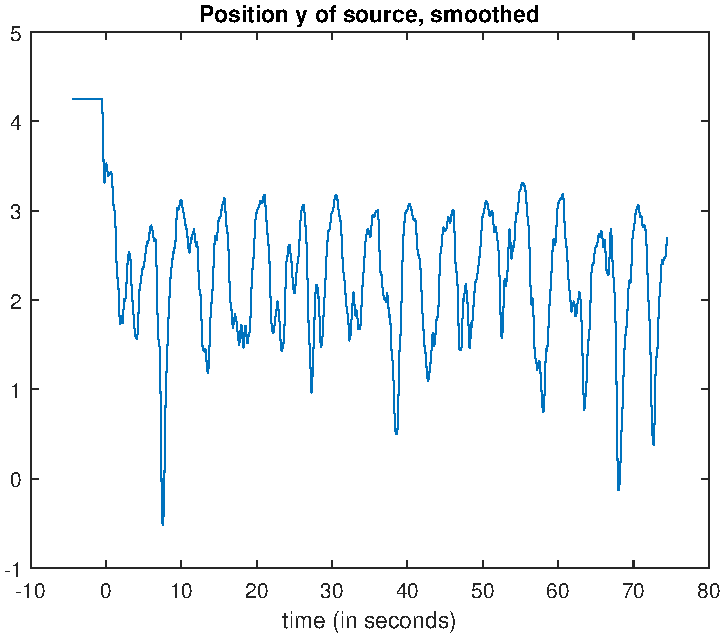
\includegraphics[width=2.5in]{y-smoothed.pdf}
    \end{center}
\end{figure}

\section{Parameter Estimation}

We will now try to fit the generated signal to the following form.
\[y=A\sin(\omega t + \phi) + b\]
To estimate the mean and amplitude of the source position, begin by observing that there
are approximately two peaks every 10 seconds. Thus I will split up the signal into windows
that are 5 seconds or 1000 samples long, which is approximately one period. I want the window
to start when the sine component of \(y\) is close to zero. I ignore the first few secondns, since
these look inaccurate due to the start of the transmission signal. Thus I chose \(t=8.75\)s
as the start of the window. Then I can find the average of the signal to compute \(b\) and half
of the difference between the maximum and the minimum to compute \(A\) during this window.
I implement this with the following code.
\begin{verbatim}
startIndex=2651;
window=1000;
N=idivide(length(y)-startIndex+1,int32(window));
A=zeros(1,N);
B=zeros(1,N);
for i=1:N
    indices=(i-1)*window+startIndex:i*window+startIndex-1;
    A(i)=(max(y(indices))-min(y(indices)))/2;
    B(i)=mean(y(indices));
end
\end{verbatim}
Next I will compute \(\omega\) by finding the period \(T\) between successive peaks and troughs of each
window and using \(\omega=\frac{2\pi}{T}\). I implement this with the following code.
\begin{verbatim}
w=zeros(1,2*(N-1));
for i=1:N-1
    indices1=(i-1)*window+startIndex:i*window+startIndex-1;
    indices2=i*window+startIndex:(i+1)*window+startIndex-1;
    tCur=tPrime(indices1);
    tNext=tPrime(indices2);
    [curMax,peakCurIndex]=max(y(indices1));
    [nextMax,peakNextIndex]=max(y(indices2));
    [curMin,troughCurIndex]=min(y(indices1));
    [nextMin,troughNextIndex]=min(y(indices2));
    period1=tNext(peakNextIndex)-tCur(peakCurIndex);
    period2=tNext(troughNextIndex)-tCur(troughNextIndex);
    w(2*i-1)=2*pi/period1;
    w(2*i)=2*pi/period2;
end
\end{verbatim}
Finally we can compute \(\phi\) by finding the difference between the peaks of our signal \(y\) and
the peaks of the non phase shifted version \(y^\prime=A\sin(\omega t)+b\). Assume that \(\phi\) is
positive, so we would want to find the next peak of \(y^\prime\) at \(t^\prime\) such
that \(t^\prime>t\) where \(t\) is the time of the peak in the current window. At our first window we have
the following expression for \(t^\prime\).
\[t^\prime = 2.25T\]
Thus we can obtain \(\phi\) as follows.
\[\phi=\frac{2.25\frac{2\pi}{\omega} - t}{\omega}\]
Each window we will add one more period to \(t^\prime\), so the following code implements this method.
\small
\begin{verbatim}
phi=zeros(1,N);
for i=1:N
    indices=(i-1)*window+startIndex:i*window+startIndex-1;
    tCur=tPrime(indices);
    [curMax,peakIndex]=max(y(indices));
    phi(i)=(2*pi*(double(i)+5/4)/mean(w)-tCur(peakIndex))/mean(w);
end
\end{verbatim}
\normalsize
I tried to do the same method with the troughs of \(y\) except with the first \(t^\prime=2.75T\), but I
found that this led to higher variance and a worse fit. Thus I stuck with only using the peaks.

\section{Results}

I obtained the following values for the constants.
\[\begin{array}{c|cc}
    & \mu & \sigma\\
    \hline
    A & 1.0625 & 0.23684\\
    b & 2.2354 & 0.14709\\
    \omega & 1.2643 & 0.14677\\
    \phi & 0.21287 & 0.44424
\end{array}\]
Plotting \(y=A\sin(\omega t + \phi) + b\) using the mean of these values against the smoothed data results
in the following plot.
\begin{figure}[H]
    \begin{center}
        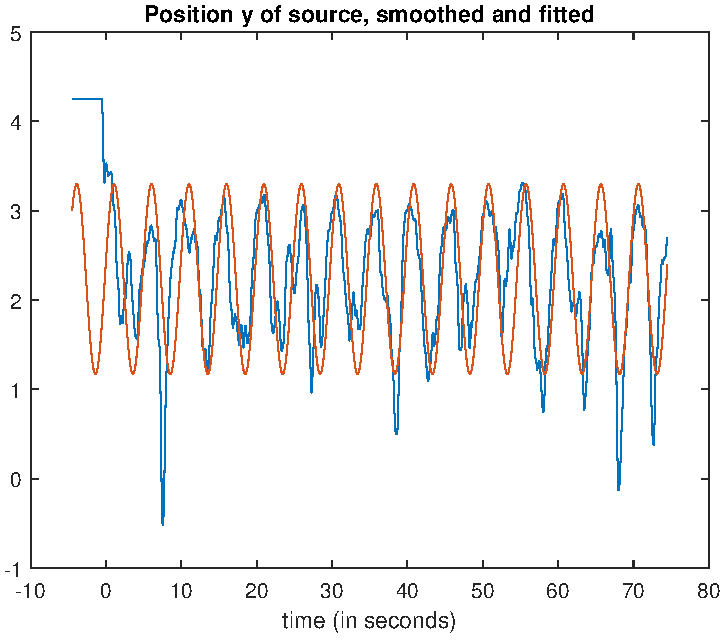
\includegraphics[width=3in]{y-fitted.pdf}
    \end{center}
\end{figure}
The first few seconds before the signal starts transmitting fully can be safely ignored. This is a fairly
good fit, and confirms that my methods worked well. The standard deviations of my results are reasonably small.
The only value with relatively high standard deviation is \(\phi\). Two standard deviations around the mean for \(\phi\)
has a range of about \(\frac{\pi}{2}\), which is somewhat high. I attempted many methods of calculating \(\phi\)
but this seems to be around the best fit that I could achieve.

\end{document}